% Modelo da Raquel - Este modelo foi baseado em: modelo-ufpr.tex,v 1.1 2003/06/30 
% incluir o pacote estilo.
% <mariane.raquel@ymail.com>

\documentclass[normaltoc, ruledheader, sumarioincompleto]{abnt}
\usepackage[brazil]{babel}
\usepackage[utf8]{inputenc}
\usepackage[T1]{fontenc}
\usepackage{indentfirst}
\usepackage{graphicx}	
\usepackage[left=3cm,right=3cm,top=3cm,bottom=3cm, pdftex]{geometry}
\usepackage{fancyhdr}
\usepackage{estilo}
\usepackage{url}
%\usepackage[alf]{abntcite}
\usepackage[square]{natbib}
\usepackage[font=small,labelfont=bf]{caption}
%\usepackage{hyperref}
\bibliographystyle{acmtrans}%{abnt-alf}  %{acm} % % Existem ainda: abbrv, acm, alpha, amsalpha, amsplain

% \documentclass[a4paper,11pt, normaltoc, pnumromarab, pagestart=fistchapter, tocpage=plain]{abnt}
% \geometry{a4paper,left=3cm,right=2cm,top=3cm,bottom=2cm}
%\usepackage[bookmarks=false]{hyperref}					%Package para hyper-referências



% --------- Início do Documento ---------

\begin{document}


\begin{titlepage}
% Logo e Universidade

\begin{flushleft} 
\begin{minipage}{0.25\textwidth}
\includegraphics[scale=0.7]{figuras/logo.png} 
\end{minipage}
\hfill
\begin{minipage}{0.7\textwidth}
\begin{flushleft}
\begin{center}
Centro Federal de Educação Tecnológica de Minas Gerais \\
Departamento de Computação \\
Engenharia de Computação
\end{center}
\end{flushleft}
\end{minipage}
\end{flushleft}

\begin{center}
% Aluno 
\vspace{1.5cm}
Mariane Raquel Silva Gonçalves

% Título
\vspace{5cm}
\begin{espacoduplo} 
\begin{Large} \textbf{ \textsc{Comparação de algoritmos paralelos de ordenação em MapReduce}}  \end{Large} \\
\end{espacoduplo}


% Orientador
\vfill
Orientadora: Profª. Drª. Cristina Duarte Murta \\[1cm]

% Data
Belo Horizonte \\ 2012 \\
 
\end{center}
\end{titlepage}
%\begin{titlepage}
% Logo e Universidade 
\begin{minipage}{0.2\textwidth}
\begin{flushleft} 
\includegraphics[scale=0.7]{figuras/logo.png} 
\end{flushleft}
\end{minipage}
\hfill
\begin{minipage}{0.7\textwidth}
\begin{flushleft}
\begin{center}
Centro Federal de Educação Tecnológica de Minas Gerais \\
Departamento de Computação \\
Engenharia de Computação
\end{center}
\end{flushleft}
\end{minipage}

\begin{center}
% Aluno 
\vspace{1.5cm}
Mariane Raquel Silva Gonçalves

% Título
\vspace{5cm}
\begin{espacoduplo} 
\begin{Large} \textbf{ \textsc{Comparação de algoritmos paralelos de ordenação em MapReduce}}  \end{Large} \\
\end{espacoduplo}

\end{center}

% Texto
\vfill
\begin{flushright}
\begin{minipage}{0.5\textwidth}
Projeto apresentado como requisito parcial à aprovação em Trabalho de Conclusão de Curso I do curso de Engenharia de Computação do CEFET-MG. 
\end{minipage}
\end{flushright}
\vfill

\begin{center}
% Orientador
Orientadora: Profª. Drª. Cristina Duarte Murta \\[1cm]

% Data
Belo Horizonte \\ 2012 \\ 
\end{center}

\end{titlepage}
%\begin{folhadeaprovacao} 

\begin{minipage}{0.2\textwidth}
\begin{flushleft} 
\includegraphics[scale=0.7]{figuras/logo.png} 
\end{flushleft}
\end{minipage}
\hfill
\begin{minipage}{0.7\textwidth}
\begin{flushleft}
\begin{center}
Centro Federal de Educação Tecnológica de Minas Gerais \\
Departamento de Computação \\
Engenharia de Computação
\end{center}
\end{flushleft}
\end{minipage}
\vfill

%\hspace{.45\textwidth} % posicionando a minipage
\framebox[.8\textwidth][c]{
\begin{minipage}{.7\textwidth}
\begin{center}
\vspace{1cm}
\textbf{Comparação de algoritmos paralelos de ordenação em MapReduce} \\
\vspace{2em}
Trabalho de Conclusão de Curso I
\vspace{2em}

\setlength{\ABNTsignthickness}{0.4pt} \setlength{\ABNTsignskip}{1cm}
\hspace*{1cm}
\assinatura{Mariane Raquel Silva Gonçalves \\ Aluna} 
\hspace*{1cm}
\assinatura{Profª. Drª. Cristina Duarte Murta \\ Orientadora}
\end{center} \end{minipage}
} \vfill
\end{folhadeaprovacao}



% Dedicatória

\pretextualchapter{}
\vspace{8cm}
\begin{flushright}
\hfill \textnormal{
Aos professores, \\
aos colegas de curso e \\
aos meus familiares, \\
dedico este trabalho.}
\end{flushright}


% Agradecimentos - é so para as pessoas que contribuiram relevantemente
% para a elaboração do trabalho

\pretextualchapter{Agradecimentos}

\begin{minipage}{\textwidth}
    Agradeço aos meus pais, pelo amor incondicional. \\
    Aos meus professores, pelos conhecimentos adquiridos. \\
     E finalmente aos colegas de curso pela convivência e trocas de experiências.
\end{minipage}

%  Epígrafe - é uma citação pertinente ao seu trabalho
%  ou que represente o seu modo de pensar.
%  Resumindo, coloque uma frase que o(a) agrade.

\pretextualchapter{}
\vspace{8cm}
\begin{flushright}
\textnormal{``Pshaw, my dear fellow, what do the public, the great unobservant public, who could hardly tell a weaver by his tooth or a compositor by his left thumb, care about the finer shades of analysis and deduction!'' \\
	\bfseries Sherlock Holmes, in ``The Adventure of the Copper Beeches``}
\end{flushright}


%\begin{resumo}

    O presente trabalho tem como objetivo criar um sistema de monitoramento escalável e robusto para telefonia móvel , utilizando \emph{smartphones} com o sistema operacional \emph{Android}. A ideia é agregar à funcionalidade 
de rastreamento, a possibilidade de execução comandos de forma remota, criando assim uma gama maior de aplicações para o sistema. Um exemplo interessante, seria no caso de roubo. Atualmente as pessoas costumam guardar 
informações pessoais e sigilosas  em seu celular, portanto seria de extremo interesse que uma vez confirmado a perda do aparelho ela pudesse apagar estas informações.
    
    \par
    \textbf{Palavras-chave:} \emph{Android}, \emph{Pattern: Command}, \emph{Java}, \emph{Google App Engine}, \emph{Computação em Nuvens},\emph{Rastreamento}, \emph{Telefonia móvel}.
\end{resumo}


\begin{abstract}
	
    This paper aims to create a scalable and robust  tracking system for the mobile phone network, using \emph{smartphones} with the \emph{Android} operational system.
The ideia is to add a functionality of execution of remote commands to the tracking system, thus creating a wider range of applications and possibilities. An sample of those new 
features would be in the theft case, because with this functionality the cellphone  owner would easily erase his private information such as contacts, messages and data. 

    \par
    \textbf{Keywords}: Android, Pattern: Command, Java, Google App Engine, Cloud Computing, Tracking, mobile network	
\end{abstract}

\sumario
%\listadefiguras
%\listadetabelas
\chapter{Introdução}
\label{cap:introducao}

\section{Definição do Problema}

A ordenação é um dos problemas fundamentais da ciência da computação e
e um dos problemas algorítmicos mais estudados. Muitas aplicações dependem de ordenações eficientes como base para seu próprio desempenho. A ordenação por si só é um problema que abrange desde sistemas de banco de dados à computação gráfica, e muitos outros algoritmos podem ser descritos em termos de ordenação  \cite{Satish:2009,Amato:1996}.  

Na última década, a quantidade de dados (de trabalho, utilizada pelos sistemas, disponíveis) aumentou várias ordens de grandeza, fazendo o processamento dos dados um desafio para a computação sequencial. Como resultado, torna-se crucial substituir a computação tradicional por computação distribuída eficiente \cite{lin:2010}. A mudança no modelo de programação sequencial para paralelo é um fato inevitável e ocorre gradualmente, desde que a indústria declarou que seu futuro está em computação paralela, com o aumento do número de núcleos dos processadores \cite{Asanovic:2009}. 

Uso crescente de computação paralela em sistemas computacionais gera a necessidade de algoritmos de ordenação inovadores, desenvolvidos para dar suporte a essas aplicações. Consequentemente, é importante desenvolver rotinas eficientes de ordenação em arquiteturas paralelas e distribuídas. 

O MapReduce é um modelo de programação paralela desenvolvido pela Google para processamento de grandes volumes de dados distribuídos em \textit{clusters} \cite{Dean:2008}. Esse modelo propõe simplificar a computação paralela, escondendo detalhes da paralelização do desenvolvedor e utilizando duas funções principais - map e reduce.
Uma das implementações mais conhecidas e utilizadas do modelo é o Hadoop \cite{Hadoop:2010}, ferramenta de código aberto, desenvolvida por Doug Cutting em 2005 e apoiada pela Yahoo!. 

O trabalho proposto por \cite{Paula:2011} apresentou uma avaliação da escalabilidade de algoritmos de ordenação paralela no modelo MapReduce. Para tal, foi desenvolvido no ambiente Hadoop o algoritmo de Ordenação por Amostragem, e seu desempenho foi avaliado em relação à quantidade de dados e ao número de máquinas utilizadas. 
Esse projeto busca continuar tal proposta, com a implementação de outros algoritmos de ordenação no mesmo ambiente, e comparação dos seus desempenhos.

%\begin{itemize}
%\item crescimento dos dados
%\item map reduce como proposta para processamento rápido e fácil de grandes quantidades de dados
%\item uso do modelo map reduce em ordenação 
%\item comparação de algoritmos de ordenação nesse modelo
%\end{itemize}



\section{Motivação}

% 1. crescimento dos dados requer mais poder computacional

O volume de dados que é produzido e manipulado (outra palavra) em indústrias, empresas e até mesmo dados pessoais aumenta a cada ano. O desenvolvimento de soluções capazes de lidar com tais volumes de dados é uma das preocupações atuais, tendo em vista a quantidade de dados processados diariamente, e o rápido crescimento desse volume de dados.
Não é fácil medir o volume total de dados armazenados digitamente, mas uma estimativa da IDC \cite{Gantz:2008} colocou o tamanho do "universo digital" em 0,18 zettabytes em 2006, e previa um crescimento dez vezes até 2011 (para 1,8 zettabytes).
 \textit{The New York Stock Exchange} gera cerca de um terabyte de novos dados comerciais por dia. O Facebook armazena aproximadamente 10 bilhões de fotos, que ocupam mais de um petabyte. \textit{The Internet Archive} armazena aproximadamente 2 petabytes de dados, com aumento de 20 terabytes por mês
\cite{Hadoop:2010}. Estima-se que dados não estruturados são a maior porção e de a mais rápido crescimento dentro das empresas, o que torna o processamento de tal volume de dados muitas vezes inviável.

%2. mais poder computacional pode ser conseguido com a) clock  e b) paralelismo
Mesmo para os computadores atuais, é um desafio conseguir lidar com quantidades de dados tão grandes. É preciso buscar soluções escaláveis, que apresentem bom desempenho em tais condições. 
As tendências atuais em \textit{design} de microprocessadores estão mudando fundamentalmente a maneira que se obtém desempenho de sistemas computacionais. 

Nos últimos 40 anos, o aumento no poder computacional deu-se, largamente, ao aumento na capacidade do hardware. 
 O fator principal dessa melhoria foi a capacidade de dobrar, a cada dois anos, o número de dispositivos microeletrônicos em uma mesma área de silício, a um custo quase constante. Esse crescimento exponencial no número de transistores presentes nos processadores é conhecida como Lei de Moore \cite{Manferdelli:2008}. 
No entanto, o aumento no número de transistores, e consequente aumento na velocidade do processador  foi limitado por questões físicas, como a dissipação do calor, que, proporcional à frequência de \textit{clock}, impõe um limite natural ao seu crescimento.
  
%3. a indústria sabe que agora só é possível trabalhar o paralelismo

Atualmente, arquitetos de têm sido forçados a recorrer a arquiteturas paralelas para continuar a fazer progressos. O aumento no desempenho virá em vez de computação paralela.
\cite{Manferdelli:2008}
  
A indústria declarou que seu futuro está em computação paralela, com o aumento crescente do número de núcleos dos processadores \cite{Asanovic:2009}.

O modelo de programação \textit{single core} (sequencial) está sendo substituído rapidamente pelo modelo \textit{multi-core} (paralelo), e com isso surge a necessidade de escrever software para sistemas com multiprocessadores e memória compartilhada \cite{Ernst:2009}.

É um caminho natural para o processamento de dados em larga escala o uso de clusters.


% 3.5 computação paralela é dificil
Arquiteturas \textit{multi-core} podem oferecer um aumento significativo de desempenho sobre as arquiteturas de núcleo único, de acordo com as tarefas paralelizadas. No entanto, muitas vezes isto exige novos paradigmas de programação para utilizar eficientemente a arquitetura envolvida \cite{Prinslow:2011}. 

% DIZER COMO É DIFICIL

% 4. com o map reduce, é possível ordenar de forma rápida e fácil
O MapReduce\cite{Dean:2008}  é um modelo de programação paralela criado pela Google para processamento de grandes volumes de dados em \textit{clusters}. Esse modelo propõe simplificar a computação paralela e ser de fácil uso, abstraindo conceitos complexos da paralelização - como tolerância a falhas, distribuição de dados e balanço de carga - e utilizando duas funções principais: map e reduce. A complexidade do algoritmo paralelo não é vista pelo desenvolvedor, que pode se ocupar em desenvolver a solução proposta. O Hadoop \cite{Hadoop:2010} é uma das implementações do MapReduce, um \textit{framework open source } desenvolvido por Doug Cutting em 2005 que provê o gerenciamento de computação distribuída.

MapReduce e sua implementação \textit{open source} Hadoop representam uma alternativa economicamente atraente oferecendo uma plataforma eficiente de computação distribuída para lidar com grandes volumes de dados e mineração de petabytes de informações não estruturadas \cite{Cherkasova:2011}.

% 5. com o crescimento dos dados no mundo, ordenar está cada vez mais complexo 

A ordenação é um dos problemas fundamentais da ciência da computação e algoritmos paralelos para classificação têm sido estudados desde o início da computação paralela.

Um grande número de aplicações paralelas possui uma fase de computação intensa, na qual uma lista de elementos deve ser ordenada com base em algum de seus atributos. Um exemplo é o algoritmo de Page Rank \cite{Page:1999} da Google: as páginas de resultado de uma consulta são classificadas de acordo com sua relevância, e então precisam ser ordenadas de maneira eficiente \cite{Kale:2010}.

% 6. a ordenação paralela pode melhorar essa tarefa

Os algoritmos ótimos existentes em arquitetura sequencial, como Quick sort e Heap Sort necessitam de um tempo mínimo \textit{(n log n)} para ordenar uma sequência de \textit{n} elementos.  [AHO 1700] 
A ordenação é um exemplo de tarefa que pode ter seu desempenho melhorado com o uso de paralelismo. Na criação de algoritmos de ordenação paralela, é ponto fundamental ordenar coletivamente os dados de cada processo individual, de forma a utilizar todas as unidades de processamento e minimizar os custos de redistribuição de chaves entre os processadores. Fatores como movimentação de dados, balanço de carga, latência de comunicação e distribuição inicial das chaves são considerados ingredientes chave para o bom desempenho da ordenação paralela, e variam de acordo com o algoritmo escolhido como solução\cite{Kale:2010}. 
No exemplo do Page Rank, o número de páginas a serem ordenadas é enorme, e elas são recolhidas de diversos servidores da Google; é uma questão fundamental escolher algoritmo paralelo com o melhor desempenho dentre as soluções possíveis.

% 7. mas algoritmos paralelos são muito dependentes de ambiente e distribuição inicial, portanto é importante avaliar o desempenho desses algoritmos
Dado o grande número de algoritmos de ordenação paralelas e uma vasta variedade de arquiteturas paralelas, é uma tarefa difícil escolher o melhor algoritmo para uma determinada máquina e instância do problema. A principal razão que a escolha é mais difícil do que em máquinas sequenciais é porque não existe um modelo teórico conhecido que pode ser aplicado para prever com precisão o desempenho de um algoritmo em arquiteturas diferentes. Assim, experimental estudos assumem uma crescente importância para a avaliação e seleção de algoritmos apropriados para multiprocessadores. Tem havido um número de estudos de implementação relatados na literatura nos últimos anos (ver, por exemplo, [5, 12]). No entanto, mais estudos são necessários antes que possamos aproximar-se do ponto onde um determinado algoritmo pode ser recomendado para uma determinada máquina com algum grau de confiança.
[Amato 1996]

%\begin{itemize}
%\item crescimento dos dados requer mais poder computacional
%\item mais poder computacional pode ser conseguido com a) clock  e b) paralelismo
%\item a indústria sabe que agora só é possível trabalhar o paralelismo
%\item ordenação é uma tarefa de grande importância
%\item com o crescimento dos dados no mundo, ordenar está cada vez mais complexo
%\item a ordenação paralela pode melhorar essa tarefa
%\item com o map reduce, é possível ordenar de forma rápida e fácil
%\item mas algoritmos paralelos são muito dependentes de ambiente e distribuição inicial, portanto é importante avaliar o desempenho desses algoritmos
%\end{itemize}

\section{Objetivos}

Os objetivos deste trabalho são:

\begin{packed_enum}
\item Estudar a programação paralela aplicada à algoritmos de ordenação;
\item Implementar um ou mais algoritmos de ordenação paralela no modelo MapReduce, com o software Hadoop;
\item Comparar duas ou mais implementações de algoritmos paralelos de ordenação.
\end{packed_enum}

O trabalho desenvolvido por ~\cite{Paula:2011} apresentou um estudo sobre a computação paralela e algoritmos de ordenação no modelo MapReduce, através da implementação do algoritmo de Ordenação por Amostragem feita em ambiente Hadoop. 

Este projeto busca continuar o estudo sobre ordenação paralela feito no trabalho citado, com a análise de desempenho dos algoritmos de ordenação ordenação por amostragem e quick sort. A análise busca compará-los com relação à quantidade de dados a serem ordenados, variabilidade dos dados de entrada e número máquinas utilizadas. 


\section{Organização do Texto}

Esse projeto está organizado em 6 capítulos. O próximo capítulo apresenta o referencial teórico para o desenvolvimento do trabalho. %,com modelos de programação paralela aplicados à ordenação. 
O capítulo ~\ref{cap:ordenacao} complementa o referencial teórico, e apresenta de maneira mais detalhada os conceitos mais importantes da ordenação em ambiente paralelo.
O capítulo ~\ref{cap:metodologia} descreve a metologia de pesquisa à ser aplicada no desenvolvimento do projeto. Os resultados preliminares obtidos até a entrega do projeto são apresentados no capítulo \ref{cap:resultados}. As conclusões obtidas até o momento e os próximos passos para a conclusão do projeto estão no ~\ref{cap:conclusao}.







%%Citações: 
%%\cite{Kale:2010} 
%%\cite{Manferdelli:2008} 
%%\cite{Dean:2008} 
%%\cite{Asanovic:2009}
%% \cite{Ernst:2009}
%% \cite{Hadoop:2010}
%% \cite{PageRank:1999}
%% \cite{Cherkasova:2011}
%% \cite{Prinslow:2011}
\chapter{Referencial Teórico}
\label{cap:referencial}

 
% computação paralela
\section{ Computação Paralela}


Com o avanço tecnólogico da última década, o volume crescente de dados sendo gerado, coletado e armazenado tornou o processamento dos dados inviável para um único computador. A quantidade de dados atualmente processados cria a necessidade de computação de alto desempenho, cujo foco sejam os dados.  Como resultado, torna-se crucial substituir a computação tradicional por computação distribuída eficiente. 
É um caminho natural para o processamento de dados em larga escala o uso de \textit{clusters} ~\cite{Lin:2010}.

\textit{Clusters} são conjuntos de máquinas, ligadas em rede, que comunicam-se através do sistema, trabalhando como se fossem uma única máquina de grande porte. 
Dentre algumas características observadas em um \textit{cluster}, é possível destacar: o baixo custo se comparado a supercomputadores; a proximidade geografica dos nós. altas taxas de transferência nas conexões entre as máquinas e o uso de máquinas em geral homogêneas \cite{Toth:2008}.

Apesar dos computadores em um \textit{cluster} não precisarem processar necessariamente a mesma aplicação, a grande vantagem de tal organização é a habilidade de cada nó processar individualmente uma fração da aplicação, resultando em desempenho que pode ser comparado ao de um supercomputador.
Em geral os computadores de \textit{clusters} são de baixo custo, o que permite que um grande número de máquinas seja interligado, garantindo desempenho e melhor custo-benefício que supercomputadores, o que apresenta grande vantagem. Outro ponto importante é que novas máquinas podem ser facilmente incorporadas  ao \textit{cluster}, tornando-o uma solução mais flexível, principalmente por ser formado por máquinas de capacidade de processamento similar.

\textit{Esta linha de pesquisa envolve vários outros conceitos relacionados à infraestrutura, como comunicação entre os nós, balanceamento de carga e outros discutidos nas próximas seções.}



// FIGURA ARQUITETURA

\subsection{ Princípios de processamento em cluster? distribuído? de grande volumes de dados? }

O processamento de grandes volumes de dados em \textit{clusters} deve ser baseado em alguns princípios para garantir a escalabilidade e o bom desempenho \cite{Bryant:2011}:



\paragraph{Tratamento de dados intrínsecos}
A coleta e manutenção dos dados deve ser funções do sistema e não tarefa dos usuários.  
O sistema deve recuperar informações atualizadas através de rede e realizar cálculos derivados como tarefas em segundo plano. Os usuários devem ser capazes de usar consultas ricos com base no conteúdo e identidade para acessar os dados. 
Mecanismos de confiabilidade, como replicação e de correção de erros devem ser incorporados como parte do sistema, de modo a garantir integridade e disponibilidade dos dados.

\paragraph{Modelo de programação paralelo de alto nível}
O desenvolvedor da aplicação deve fazer uso de primitivas de programação de alto nível, capazes de expressar formas naturais de paralelismo, que não incluam cofigurações específicas de uma máquina. O trabalho de Mapear essas computações para a máquina de forma eficiente deve ficar a cargo do sistema, compilador e runtime.

\paragraph{Acesso interativo} 
Os usuários devem ser capazes de executar programas de forma interativa, com variação dos requisitos de computação e armazenamento O sistema deve responder a consultas e cálculos simples rapidamente, e responder aos complexos sem degradar o desempenho geral. Para suportar a computação interativa, deve haver oferta de recursos. O custo consequente do aumento dos recursos ofertados pode ser justificado com base no aumento da produtividade dos usuários do sistema.


\paragraph{Mecanismos escaláveis para garantir alta confiabilidade e disponibilidade}
Um sistema para computação de grandes volumes de dados deve implementar mecanismos de confiabilidade, no qual os dados originais e intermediários são armazenados de forma redundante. Isso permite que no caso de falhas de componente ou dados seja possível refazer a computação. Além disso, a máquina deve identificar e desativar automaticamente componentes que falharam, de modo a não prejudicar o desempenho do sistema e se manter sempre disponível. 


Grandes empresas de serviços de Internet - como Google, Yahoo, Facebook e Amazon - buscam soluções para processamento de dados em grandes conjuntos de máquinas que atendam as características descritas. Com um software que provê tais características é possível alcançar alto grau de escalabilidade e custo-desempenho. 

Dentre as principais propostas está o modelo MapReduce e sua implementação Hadoop, que são soluções escaláveis, capazes de processar grandes volumes de dados, com alto nível de abstração para distribuir a aplicação e mecanismos de tolerância a falhas.
A próxima seção apresenta com mais detalhes o modelo e suas características.

%
%
%\textit{modelos de computação paralela (memória compartilhada, distribuida, threads, paralelismo de dados e Map Reduce)}
%
% More precise simulations or the simulations of larger problems need greater and greater computing power and memory space. In the last decades, high-performance research included new developments in parallel hard- ware and software technologies, and a steady progress in parallel high-performance computing can be observed.
% Multicore architectures in the form of single multicore processors, shared mem- ory systems of several multicore processors, or clusters of multicore processors with a hierarchical interconnection network will have a large impact on software development.
%
%Parallel programming models provide methods to support the parallel programming.
%
%parallel programming techniques that are neces- sary for developing efficient programs for multicore processors as well as for par- allel cluster systems
%
%
%The goal of a programming model is to provide a mechanism with which the programmer can specify parallel programs. To do so, a set of basic tasks must be supported. A parallel program specifies computations which can be executed in par- allel.
%
%The programming model is at the next higher level of abstraction and describes a parallel computing system in terms of the semantics of the programming lan- guage or programming environment. A parallel programming model specifies the programmer’s view on parallel computer by defining how the programmer can code an algorithm. This view is influenced by the architectural design and the language, compiler, or the runtime libraries and, thus, there exist many different parallel pro- gramming models even for the same architecture. There are several criteria by which the parallel programming models can differ:
%• the level of parallelism which is exploited in the parallel execution (instruction level, statement level, procedural level, or parallel loops);
%• theimplicitoruser-definedexplicitspecificationofparallelism;
%• thewayhowparallelprogrampartsarespecified;
%• the execution mode of parallel units (SIMD or SPMD, synchronous or asyn-
%chronous);
%• themodesandpatternofcommunicationamongcomputingunitsfortheexchange
%of information (explicit communication or shared variables);
%• synchronizationmechanismstoorganizecomputationandcommunicationbetween
%parallel units.
%
%For the software developer, the new hardware development toward multicore architectures is a challenge, since existing software must be restructured toward parallel execution to take advantage of the additional computing resources. In partic- ular, software developers can no longer expect that the increase of computing power can automatically be used by their software products. Instead, additional effort is required at the software level to take advantage of the increased computing power.
%
%There is much research going on in the area of parallel programming languages and environments with the goal of facilitating parallel programming by providing support at the right level of abstraction.


\section{MapReduce}
O MapReduce é um modelo de programação paralela criado pela Google para processamento de grandes volumes de dados em \textit{clusters}. Esse modelo propõe simplificar a computação paralela e ser de fácil uso, abstraindo conceitos complexos da paralelização - como tolerância a falhas, distribuição de dados e balanço de carga - e utilizando duas funções principais: Map e Reduce. A complexidade do algoritmo paralelo não é vista pelo desenvolvedor, que pode se ocupar em desenvolver a solução proposta \cite{Dean:2008}.

Esse modelo de programação é inspirado em linguagens funcionais, tendo como base as primitivas Map e Reduce.
Os dados de entrada são específicos para cada aplicação, e descritos pelo usuário. A saída é um conjunto de pares no formato (chave, valor).
A função Map é aplicada aos dados de entrada e produz uma lista intermediária de pares (chave, valor). Todos os valores intermediários associados a uma mesma chave são agrupados e enviados à função Reduce.
A função Reduce é então aplicada para todos os pares intermediários com a mesma chave. A função combina esses valores para formar um conjunto menor de resultados.
Tipicamente, há apenas zero ou um valores de saída em cada função Reduce.

O pseudocódigo a seguir apresenta um exemplo de uso do MapReduce, cujo objetivo é contar a quantidade de ocorrências de cada palavra em um documento. A função Map recebe como valor uma linha do documento texto, e como chave o número da linha. Para cada palavra encontrada na linha recebida, a função emite a palavra e a contagem de uma ocorrência. A função Reduce, recebe como chave uma palavra, e uma lista dos valores emitidos pela função Map, associados com a palavra questão. As ocorrências da palavra são agrupadas e a função retorna palavra e seu total de ocorrências.

\begin{lstlisting}[label=some-code,caption=some-code]
Function Map (Integer chave, String valor):
	#chave: número da linha no arquivo.
	#valor: texto da linha correspondente.
	listaDePalavras = split (valor)
	for palavra in listaDePalavras:
		emit (palavra, 1)
Function Reduce (String chave, Iterator valores):
	#chave: palavra emitida pela função Map.
	#valores: conjunto de valores emitidos para a chave.
	total = 0
	for v in valores:
		total = total + 1
	emit (palavra, total)
\end{lstlisting}

A Figura \ref{fig:MapReduceexemplo} ilustra o fluxo de execução para este exemplo. A entrada é um arquivo contendo as linhas "exemplo conta palavras" e "hadoop exemplo palavras".

\begin{figure}[htb]
\centering
%trim left, bottom, right and top
\includegraphics[trim=0cm 9cm 0cm 1cm, width=\textwidth]{figuras/MapReduceExemplo.pdf}
\caption{Fluxo simplificado da contagem de palavras com o MapReduce}
\label{fig:MapReduceexemplo}
\end{figure}

\subsubsection{Arquitetura do MapReduce}
O MapReduce é constituído de uma arquitetura com dois tipos principais de nós: \textit{Master} e \textit{Worker}. O nó mestre tem como função atender requisições de execução dos usuários, gerenciá-las, criar tarefas e distribuí-las entre os nós trabalhadores, que executam as tarefas com base nas funções Map e Reduce definidas pelo usuário.
%Como é possível perceber, trata-se de uma típica arquitetura mestre-escravo (do inglês master-slave) (DUBREUIL; GAGNÉ; PARIZEAU, 2006).
A arquitetura também é inclui um sistema de arquivos distribuídos, onde ficam armazenados os dados de entrada e intermediários.
%Para evitar a transferência excessiva de dados, os \textit{workers} do MapReduce são também nós do sistema de arquivos.


% }

\subsubsection{Visão geral do fluxo de execução}


As chamadas da função Map são distribuídas automaticamente entre as diversas máquinas através do particionamento dos dados de entrada em \textit{M} conjuntos. Cada conjunto pode ser processado em paralelo por diferentes máquinas. As chamadas da função Reduce são distribuídas pelo do particionamento do conjunto intermediário de pares em \textit{R} partes. O número de partições \textit{R} pode ser definido pelo usuário.

A Figura \ref{fig:MapReduceoverview} ilustra uma o fluxo de uma execução do modelo MapReduce \cite{Dean:2008}. A sequência de ações descrita a seguir explica o que ocorre em cada um dos passos. A numeração dos itens a seguir corresponde à numeração da figura.



 \begin{figure}[!htb]
 \centering
%trim left, bottom, right and top
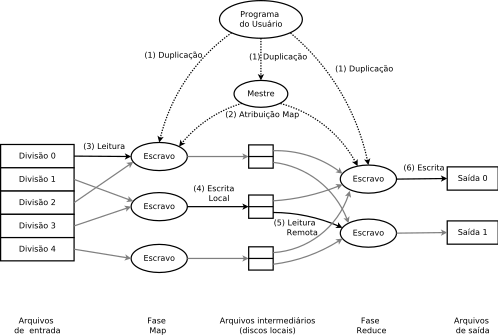
\includegraphics[trim=0cm 2cm 0cm 1cm, width=\textwidth]{figuras/MapReduceOverflow.pdf}
\caption{Visão geral do funcionamento do modelo MapReduce.}
\label{fig:MapReduceoverview}
\end{figure}



\begin{enumerate}
\item A biblioteca MapReduce no programa do usuário primeiro divide os arquivos de entrada em M pedaços. Em seguida, iniciam-se muitas cópias do programa em um cluster de máquinas.

\item Uma das cópias do programa é especial: o mestre (\textit{master}). Os demais são trabalhadores (escravos, slaves) cujo trabalho é atribuído pelo mestre. Existem M tarefas Map e R tarefas Reduce a serem atribuídas. O mestre atribui aos trabalhadores ociosos uma tarefa Map ou uma tarefa Reduce.

\item Um trabalhador que recebe uma tarefa Map lê o conteúdo do fragmento de entrada correspondente. Ele analisa pares (chave, valor), a partir dos dados de entrada e encaminha cada par para a função Map definida pelo usuário. Os pares (chave, valor) intermediários, produzidos pela função Map, são colocados no buffer de memória;

\item Um trabalhador que recebe uma tarefa Map lê o conteúdo do fragmento de entrada correspondente. Ele analisa pares (chave, valor), a partir dos dados de entrada e encaminha cada par para a função Map definida pelo usuário. Os pares (chave, valor) intermediários, produzidos pela função Map, são colocados no buffer de memória;

\item Periodicamente, os pares colocados no buffer são gravados no disco local, divididos em regiões R pela função de particionamento. As localizações desses pares bufferizados no disco local são passadas de volta para o mestre, que é responsável pelo encaminhamento desses locais aos trabalhadores Reduce;

\item Quando um trabalhador Reduce é notificado pelo mestre sobre essas localizações, ele usa chamadas de procedimento remoto para ler os dados no buffer, a partir dos discos locais dos trabalhadores Map. Quando um trabalhador Reduce tiver lido todos os dados intermediários para sua partição, ela é ordenada pela chave intermediária para que todas as ocorrências da mesma chave sejam agrupadas. Se a quantidade de dados intermediários é muito grande para caber na memória, um tipo de ordenação externa é usado;

\item O trabalhador Reduce itera sobre os dados intermediários ordenados e, para cada chave intermediária única encontrada, passa a chave e o conjunto correspondente de valores intermediários para função Reduce do usuário. A saída da função Reduce é anexada a um arquivo de saída final para essa partição Reduce;

\item Quando todas as tarefas Map e Reduce são concluídas, o mestre acorda o programa do usuário. Neste ponto, a chamada MapReduce no programa do usuário retorna para o código do usuário.
              	        	
\end{enumerate}


\subsection{Hadoop}
Uma das implementações mais conhecidas do MapReduce é o Hadoop, desenvolvido por Doug Cutting em 2005 e mantido pela Apache Software Foundation. O Hadoop é uma implementação código aberto em Java do modelo criado pela Google, que provê o gerenciamento de computação distribuída, de maneira escalável e confiável \cite{Hadoop:2010}.

Facebook, Yahoo! e eBay utilizam o ambiente Hadoop em seus \textit{clusters} para processar diariamente terabytes de dados e logs de eventos para detecção de spam, \textit{business intelligence} e diferentes tipos de otimização \cite{Cherkasova:2011}.

O modelo MapReduce foi criado para permitir o processamento em conjuntos de centenas de máquinas de maneira transparente, o que significa que o usuário não deve ser preocupar com mecanismos de tolerância a falhas, que deve ser provido pelo sistema \cite{Dean:2008}. 
Um dos principais benefícios do Hadoop é a sua capacidade de lidar com falhas, sejam de disco, processos, ou de nós, e permitir que o trabalho do usuário possa ser concluído.

O sistema é capaz de verificar e substituir nós quando ocorre alguma falha. O nó mestre envia mensagens periódicas aos demais nós para verificar seu estado. Se nenhuma resposta é recebida, o mestre identifica que houve uma falha neste nó. 
As tarefas que não foram executadas são reescalonadas para os demais nós. O mecanismo de replicação garante que sempre haja um número determinado de cópias dos dados, e caso um dos nós de armazenamento seja perdido, os demais se encarregam de realizar uma nova replicação \cite{Hadoop:2010}.



\subsubsection{Sistema de Arquivos Distribuídos}


O \textit{ Hadoop Distributed File System} (HDFS) é um sistema de arquivos distribuído desenvolvido para armazenar grandes conjuntos de dados e ser altamente tolerante a falhas \cite{Hadoop:2010}.
A plataforma Hadoop suporta diversos sistemas de arquivos distintos, como Amazon S3 (Native e Block-based), CloudStore, HAR, sistemas mantidos por servidores FTP e HTTP, Local (destinado a unidades de armazenamento conectadas localmente), mas fornece o HDSF como sistema de arquivos padrão.

A arquitetura do HDFS também é do tipo mestre-escravos.
O nó mestre (\textit{NameNode}) é responsável por manter e controlar todos os metadados do sistema de arquivos e gerenciar a localização dos dados. Também é responsável por outras atividades, como por exemplo, balanceamento de carga, \textit{garbage collection}, e atendimento a requisições dos clientes.
Os nós escravos (\textit{DataNode}) são responsáveis por armazenar e transmitir os dados aos usuários que os requisitarem.

A Figura \ref{fig:hdfs} ilustra a arquitetura do sistema de arquivos distribuídos.
O \textit{Namenode} gerencia e manipula todas as informações dos arquivos, tal como a localização e o acesso. Os \textit{Datanodes} se encarregam da leitura e escrita das informações nos sistemas de arquivos cliente. Os conceitos de nó \textit{Master} e \textit{Worker} do MapReduce, são respectivamente denominados JobTracker e TaskTracker no Hadoop.
\begin{figure}[htb]
\centering
%trim left, bottom, right and top
\includegraphics[trim=0cm 6cm 0cm 2cm, width=0.6\textwidth]{figuras/HadoopCluster.pdf}
\caption{Visão abstrata do cluster.}
\label{fig:hdfs}
\end{figure}

O HDFS incorpora funcionalidades que têm grande impacto no desempenho geral do sistema.
Uma delas é conhecida como \textit{rack awareness}. Com esse recurso, o sistema de arquivos é capaz de identificar os nós escravos que pertencem a um mesmo \textit{rack}, e distribuir as réplicas de maneira mais inteligente, aumentando a performance e confiabilidade do sistema.
A outra é a distribuição dos dados. O sistema de arquivos busca manter um balanceamento na ocupação das unidades de armazenamento, e o \textit{framework}, busca atribuir tarefas a um \textit{worker} que possua, em sua unidade de armazenamento local, os dados que devem ser processados.
Assim, quando executa-se grandes operações MapReduce com um número significante de nós, a maioria dos dados são lidos localmente e o consumo de banda é mínimo.





\section{Ordenação}


%
%Um grande número de aplicações paralelas possui uma fase de computação intensa, na qual uma lista de elementos deve ser ordenada com base em algum de seus atributos. Um exemplo é o algoritmo de Page Rank \cite{Page:1999} da Google: as páginas de resultado de uma consulta são classificadas de acordo com sua relevância, e então precisam ser ordenadas de maneira eficiente \cite{Kale:2010}.
%No exemplo do Page Rank, o número de páginas a serem ordenadas é enorme, e elas são recolhidas de diversos servidores da Google; é uma questão fundamental escolher algoritmo paralelo com o melhor desempenho dentre as soluções possíveis.
%
%Na criação de algoritmos de ordenação paralela, é ponto fundamental ordenar coletivamente os dados de cada processo individual, de forma a utilizar todas as unidades de processamento e minimizar os custos de redistribuição de chaves entre os processadores.
%\label{cap:ordenacao}
%
%\begin{itemize}
%\item importância da ordenação paralela
%\item formas de ordenação: memória e disco
%\item grandes dados: apenas disco
%\item grandes dados: problematização (tempo, limite de memória)
%\item grandes dados: sort benchmark
%\end{itemize}
%
%
%\begin{itemize}
%\item algoritmos de ordenação paralelos
%\item funcionamento geral
%\item condições / ingredientes / limites
%\item diferentes algoritmos para diferentes aplicações
%\item descrição de algoritmos (e diagramas): sample sort, quick sort
%
%\end{itemize}



A ordenação em memória interna é caracterizada pelo armazenamento de todos os registros na memória principal, onde seus acessos são feitos diretamente pelo processador. Essa ordenação é possível apenas quando a quantidade de dados é pequena o suficiente para ser armazenada em memória. 

Quando a ordenação é feita em um grande conjunto de dados, que não podem ser armazenados em memória principal a ordenação é chamada externa. Apesar do problema nos dois casos ser o mesmo (rearranjar os registros de um arquivo em ordem ascendente ou descendente), não é possível usar as mesmas estratégias da ordenação interna, pois o acesso aos dados é feito em discos, cujo tempo de acesso é muito superior ao da memória principal.  %[Ziviani 2007, Knuth 1973].

Na ordenação externa, os itens que não estão na memória principal devem ser buscados em memória secundária e trazidos para a memória principal, para assim serem comparados. Esse processo se repete inúmeras vezes, o que o torna lento, uma vez que os processadores ficam grande parte do tempo ociosos à espera da chegada dos dados à memória principal para serem processados. Por esse motivo, a grande ênfase de um método de ordenação externa deve ser na minimização do número de vezes que cada item é transferido entre a memória interna e a memória externa. Além disso, cada transferência deve ser realizada de forma tão eficiente quanto as características dos equipamentos disponíveis permitam \cite{Ziviani:2007}.



\section{Algoritmos de Ordenação Paralela}

A ordenação paralela é o processo  de ordenação feito através de múltiplas unidades de processamento, que trabalham em conjunto para ordenar a sequência de entrada. O conjunto inicial é divido em sub-conjuntos disjuntos, que são associados a uma única unidade de processamento. A sequência final ordenada é obtida a partir da composição dos sub-conjuntos ordenados. É um ponto fundamental do algoritmo que a ordenação feita por cada processo individual seja organizada de tal forma que todas as unidades de processamento estejam trabalhando, enquanto o custo de redistribuição de chaves entre os processadores é minimizado. 



\subsection{Condições de implementação de algoritmos paralelos de ordenação}
 
Diversas soluções de ordenação podem ser consideradas ao implementar um algoritmo de ordenação em ambiente paralelo. Cada uma delas atende a cenário, tipo de entrada, plataforma ou arquitetura particulares. Dessa forma, ao implementar algoritmos de ordenação paralela, é importante considerar certas condições que interferem no desempenho final do algoritmo, relacionadas tanto ao ambiente de implementação, quanto ao conjunto de dados que deve ser ordenado. As principais questões a serem analisadas são \cite{Kale:2010} :

\begin{itemize}
\item \textbf{Habilidade de explorar distribuições iniciais parcialmente ordenadas:}
Alguns algoritmos podem se beneficiar de cenários nos quais a sequência de entrada dos dados é mesma, ou pouco alterada. Nesse caso, é possível obter melhor desempenho ao realizar menos trabalho e movimentação de dados.
Se a alteração na posição dos elementos da sequência é pequena o suficiente, grande parte dos processadores mantém seus dados iniciais e precisa se comunicar apenas com os processadores vizinhos.

\item \textbf{Movimentação dos dados:}
A movimentação de dados entre processadores deve ser mínima durante a execução do algoritmo. Em um sistema de memória distribuída, a quantidade de dados a ser movimentada é um ponto crítico, pois o custo de troca de dados pode dominar o custo de execução total e limitar a escalabilidade.

\item \textbf{Balanceamento de carga:}
O algoritmo de ordenação paralela deve assegurar o balanceamento de carga ao distribuir os dados entre os processadores. Cada processador deve receber uma parcela equilibrada dos dados para ordenar, uma vez que o tempo de execução da aplicação é tipicamente limitada pela execução do processador mais sobrecarregado.

\item \textbf{Latência de comunicação:}
A latência de comunicação é definida como o tempo médio necessário para enviar uma mensagem de um processador a outro.
Em grandes sistemas distribuídos, reduzir o tempo de latência se torna muito importante.

\item \textbf{Sobreposição de comunicação e computação:}
Em qualquer aplicação paralela, existem tarefas com focos em computação e comunicação. A sobreposição de tais tarefas permite que sejam feitas tarefas de processamento e ao mesmo tempo operações de entrada e saída de dados, evitando que os recursos fiquem ociosos durante o intervalo de tempo necessário para a transmissão da carga de trabalho.

\end{itemize}


Além das condições relacionadas à implementação do algoritmo em ambiente paralelo, existem outras condições necessárias, relacionadas principalmente às propriedades do conjunto de elementos a ser ordenado. Considerando um conjunto de elementos $ \tau = {k1, k2, ... , kn} $ distribuído entre $p$ processadores, é que preciso durante a execução de qualquer algoritmo de ordenação paralela: 

\begin{enumerate}
\item Todas as chaves da sequencia inicial sejam preservadas, ou seja, não se perca nenhuma chave durante a distribuição entre os processadores.
\item  O conjunto de chaves seja particionada em $p$ sub-conjuntos mutualmente exclusivos, sem nenhuma chave duplicada.
\item O conjunto de todas as chaves satisfaça as propriedades de um conjunto parcialmente ordenado.
\end{enumerate}

Após o conjunto estar ordenado, é preciso que pós condições sejam satisfeitas:
\begin{enumerate}

\item Todas as chaves da sequencia inicial foram preservadas.
\item Todas as chaves de cada processador estão ordenadas em ordem crescente.
%$\forall i $ tal que $i < p$, a
\item A maior chave no processador $p_{i}$ é inferior ou igual ao menor chave no processador $p_{i+1}$.
\item A saída resultante deve ser uma sequência de chaves que satisfaça as propriedades de um conjunto totalmente ordenado.

\end{enumerate}

\subsection{Fluxo de execução geral}

Na execução de um algoritmo de ordenação paralela, podem ser identificadas algumas tarefas principais,  normalmente realizadas de forma sequencial, que todos os algoritmos precisam realizar em algum momento \cite{Kale:2010}: 
%visto pela perspectiva da comunicação, pode ser generalizada, uma vez que estão submetidos às mesmas limitações. 
%A fim de fazer uma generalização sobre o fluxo de controle de algoritmos de ordenação, algumas tarefas podem ser definidas, de maneira superficial, como se segue:

%De forma geral, todos os algoritmos de ordenação paralela executam três funções: 

\begin{itemize}
\item \textbf{Ordenação Local:} as chaves em cada processador são normalmente ordenadas inicialmente, ou ordenadas em grupos, em algum ponto da execução.
\item \textbf{Bucketing(?):} muitas vezes é necessário colocar as chaves em grupos, a fim de enviá-las a outros processadores ou calcular histogramas.
\item \textbf{Agrupamento:} as chaves são ordenadas em sub-sequências e precisam ser combinadas em uma sequência completa.
\end{itemize}



// TEXTO


1. Realizar processamento local. 
\\2. Coletar informações relevantes de distribuição de todos os processadores. 
\\3. Em um único processador, inferir uma divisão de chaves a partir das informações coletadas. 
\\4. Transmitir aos outros processadores a divisão dos elementos
\\5. Realizar processamento local. 
\\6. Mover os dados de acordo com os elementos de divisão. 
\\7. Realizar processamento local. 
\\8. Se a divisão foi incompleta (nem todos SPTR definido), retornar ao passo 1.


%\begin{lstlisting}[label=passos,caption=Passos gerais da ordenação paralela]
%Realizar processamento local. 
%Coletar informações relevantes de distribuição de todos os processadores. 
%Em um único processador, inferir uma divisão de chaves a partir das informações coletadas. 
%Transmitir aos outros processadores a divisão dos elementos
%Realizar processamento local. 
%Mover os dados de acordo com os elementos de divisão. 
%Realizar processamento local. 
%Se a divisão foi incompleta (nem todos SPTR definido), retornar ao passo 1.
%\end{lstlisting}

%This analysis gives us a few insights towards communica- tion efficiency of parallel sortng algorithms. First, there are two major communication functions, figuring out a global splitting vector and transposing the data to the proper pro- cessors. The second insight is that most algorithms have multiple stages of local work and it can be very beneficial to try to overlap this local work with the communication. 
%Finally, if overlap can be achieved between local work and the third step (sequential splitter determination), a proces- sor can be reserved for the splitting work, shortening the critical path.
%The cost of the communication a parallel sorting algorithm needs (to infer the splitting and move the data) and the cost of local work that can be overlapped with, gives us a very good idea of the comparative parallel scalability of parallel sorting algorithms.

De acordo com essa generalização, é possível identificar pontos que se relacionam diretamente com as condições que limitam o desempenho dos algoritmos de ordenação paralela, e fornecem ideias para a análise de eficiência da comunicação dos algoritmos. 
Primeiro, há duas funções principais de comunicação: descobrir um vetor de divisão global e enviar os dados para os processadores adequados. 
Em segundo lugar, a maioria dos algoritmos têm múltiplos estágios de computação local e pode ser muito vantajoso sobrepor este processamento local e a comunicação. 
%Finalmente, se é possível realizar sobreposição entre o processamento local e a determinação do vetor de divisão, um processador pode ser reservado para o trabalho de divisão, encurtando o caminho crítico. 
O custo da comunicação necessária em um algoritmo (para determinar a divisão e mover os dados) e o custo do processamento local que pode ser sobreposto à essa comunicação é um bom indicativo para comparação da escalabilidade dos algoritmos de ordenação paralela.

%4.1.1 General terminology
%The following terms will be used repeatedly throughout the solution section.
%• n - total number of elements to be sorted.
%• p - number of processing units
%• Π[1,p] - unsorted initial sequences. Processing unit k posseses Πk for k ∈ [1, p].
%• len[1,p] - length of initial sequences. Πk has length k fork∈[1,p].
%• Ξ[1,p] - sorted final sequences. Processing unit k poss- esesΞk fork∈[1,p].
%• flen[1,p] - length of final sequences. Ξk has length flenk fork∈[1,p].
%• threshold - the maximum number of extra keys each
%processor can end up with. More precisely, for all k ∈
%[1, p], f lenk ≤ n + threshold. p

%4.1.2 Splitting of data
%A fundamental problem of parallel sorting is ensuring that each Ξk has a continuous portion of the entire key set. This requirement is necessary to achieve globally sorted order over all processors. The requirement could be rephrased to say that for k ∈ [2,p − 1], Ξk has all existing keys in the range [Sptr[k − 1], Sptr[k]], Ξ1 has all keys smaller than Sptr[1] and, Ξp has all keys larger than Sptr[p − 1]. Sptr is commonly referred to as a splitting vector and has length p−1.
%Most modern parallel sorting algorithms find Sptr explicitly in order to determine what processor each key belongs on. The difficulty lies in that Sptr directly dictates the load balance of the final sequence sizes. As previously mentioned,
%
%f lenk should be smaller than n + threshold for all k ∈ [1, p]. p
%It is therefore necessary to find a splitting vector, Sptr, such that for each of p key ranges generated by elements Sptr, the number of existing keys in the range is smaller than
%n +threshold. p
%At a high level, we can gain the insight that a splitting vector needs to properly relate the distribution of keys within the key range with the corresponding key values.
%There are three commonly used methods for determining the splitting vector, Sptr:
%1. Pre-emptive: Use application-level knowledge to es- tablish Sptr directly. Or, simply assume Sptr to be uniform.
%2. Sample [7] : draw a sample from the global key set and select Sptr from the sample.
%3. Histogram [8]: make a naive guess at Sptr, then iter- atively adjust it by computing how many keys belong to each range.
%Many parallel sorting algorithms use modified versions of these techniques but most use at least one at a high level. Notably, some algorithms do not determine Sptr all at once but rather in multiple iterations or levels of recursion.



\subsection{Sample Sort}

O algoritmo \textit{Sample Sort}, ou Ordenação por Amostragem, é um método de ordenação baseado na divisão do arquivo de entrada em subconjuntos, de forma que as chaves de um subconjunto $i$ sejam menores que as chaves do subconjunto $i+1$. Após a divisão, cada subconjunto é enviado a um processador, que ordena os dados localmente. Ao final, todos os subconjuntos são concatenados e formam um arquivo globalmente ordenado.

Nesse algoritmo, o ponto chave é dividir as partições de maneira balanceada, para que cada processador receba aproximadamente a mesma carga de dados. Para isso, é preciso estimar o número de elementos que devem ser destinados a uma certa partição, que é feita através da amostragem das chaves do arquivo original. Essa estratégia baseia-se na análise de um subconjunto de dados, denominado amostra, ao invés de todo o conjunto, para estimar a distribuição de chaves e, assim, construir partições balanceadas.

Existem três tipos de estratégias de amostragem: \textit{SplitSampler}, \textit{IntervalSampler} e \textit{RandomSampler}. O \textit{SplitSampler} seleciona os $n$ primeiros registros do arquivo para formar a amostra. O \textit{IntervalSampler} cria a amostra com a seleção de chaves em intervalos regulares no arquivo. No \textit{RandomSampler}, a amostra é constituída por chaves selecionadas aleatoriamente no conjunto. A melhor estratégia de amostragem depende diretamente dos dados de entrada. O \textit{SplitSampler} não é recomendado para arquivos quase ordenados, pois as chaves selecionadas serão as iniciais, que não são representativas do conjunto como um todo. Nesse caso, a melhor escolha é o \textit{IntervalSampler} pelo fato de selecionar chaves que representam melhor a distribuição do conjunto. O \textit{RandomSampler} é considerado um bom amostrador de propósito geral [White 2009], e foi utilizado na implementação do algoritmo feito por Pinhão (2011) e utilizado neste trabalho.
Para criar a amostra, o \textit{RandomSampler} necessita de alguns parâmetros, como a probabilidade de escolha de uma chave, o número máximo de amostras a serem selecionadas para realizar a amostragem e o número máximo de partições que podem ser utilizadas.

// descrever o algoritmo em Map Reduce
%Após a formação das amostras, são definidos os limites para as partições, isto é, o intervalo de valores compreendido por cada partição. A quantidade de limites amostrados (qla) é determinada pelo equação: qla = np - 1, onde np é o número de partições (np = nc x nmaq, sendo nc o número de cores e nmaq o número de máquinas). As informações das partições são armazenadas em um arquivo e transmitidas para as máquinas participantes por meio de cache distribuído.
%

%A Figura 4.6 apresenta um esquema da estrutura de funcionamento do algoritmo, quando implementado em MapReduce no ambiente Hadoop. O algoritmo pode ser di- vidido em duas fases: Map e Reduce.
%
%Na fase Map, os arquivos de entrada são lidos, ocorre a formação do vetor inicial e dos pares (chave, valor) dos valores lidos (passos 1.1 e 1.2). Depois disso, os dados são divididos em partições cujo número é determinado pelo número de máquinas e seus núcleos de processamento (passo 1.3). No exemplo apresentado, são utilizados dois núcleos de pro- cessamento (cores). Portanto, existem duas partições e, dessa forma, deve ser escolhido apenas um limite para as partições. Esse limite é definido por meio da seleção do ele- mento que melhor representa a distribuição de chaves na amostra formada pela estratégia RandomSampler. Para esse exemplo o limite escolhido foi o número 13, o que implica que em uma partição estarão valores menores e iguais a 13 e, na outra, valores maiores que 13. Por meio de cache distribuído, as informações das partições são transmitidas para as máquinas participantes e os dados particionados. Cada partição é então atribuída a uma tarefa Reduce (processador) diferente.
%
%Na fase Reduce, os dados são ordenados localmente (passo 2.1), ou seja, em cada processador os dados são ordenados na memória interna. Para essa ordenação, avalia-se a profundidade da árvore de recursão e, se ela for baixa, utiliza-se o algoritmo QuickSort. Caso contrário, o HeapSort é utilizado [White 2009]. Após isso, os dados retornam para a máquina master, onde são concatenados, formando o vetor ordenado.O balanceamento das partições, ou seja, a formação de partições aproximadamente iguais no tamanho é muito importante para o algoritmo de Ordenação por Amostragem, pois evita que os tempos de ordenação sejam dominados por um único processador. Em outras palavras, o equilíbrio das partições reduz a possibilidade de que um processador esteja ocioso, enquanto outro processador está sobrecarregado, situação que comprometeria o desempenho do algoritmo [White 2009].

\subsection{Quick Sort}

 
\chapter{Desenvolvimento}
\label{cap:desenvolvimento}

\section{Metodologia}

A primeira fase do projeto foi destinada ao estudo mais detalhado da computação paralela, em especial dos algoritmos de ordenação paralela, do modelo MapReduce e da plataforma Hadoop. Foram realizados testes de ordenação com os \textit{benchmarks} TeraSort e Sort, e com os exemplos disponibilizados pelo Hadoop. Após esses testes, foram realizados testes com o algoritmo Ordenação por Amostragem do trabalho de Pinhão (2011), mas com com a inclusão das distribuições Normal e Pareto. O passo seguinte foi conhecer detalhadamente o algoritmo paralelo a ser implementado. No próximo semestre serão definidas as estratégias para sua implementação em ambiente Hadoop e realizados os testes. 

O algoritmo implementado deve ser cuidadosamente avaliado para verificar um funcionamento adequado com diferentes entradas e número de máquinas. Dessa forma, foram realizados experimentos para testes de desempenho dos algoritmos com relação à quantidade de máquinas, quantidade de dados e conjunto de dados.  Os resultados obtidos foram analisados a fim de permitir comparar a desempenho dos algoritmos em cada situação. 
 

\section{Infraestrutura}

A infraestrutura necessária ao desenvolvimento do projeto foi fornecida pelo Laboratório de Redes e Sistemas (LABORES) do Departamento de Computação (DECOM). O laboratório possui um \textit{cluster} formado por cinco máquinas Dell Optiplex 380, que foram utilizados na realização dos testes dos algoritmos. Os algoritmos serão desenvolvidos em linguagem Java, de acordo com o modelo MapReduce, no ambiente Hadoop. 

Cada máquina do \textit{cluster} apresenta as seguintes características:
\begin{packed_enum}
\item Processador Intel Core 2 Duo de 3.0 GHz
\item Disco rígido SATA de 500 GB 7200 RPM
\item Memória RAM de 4 GB
\item Placa de rede Gigabit Ethernet
\item Sistema operacional Linux Ubunbu 10.04 32 bits %(kernel 2.6.\textbf{XX})
\item Sun Java JDK 1.6.0 19.0-b09 
\item Apache Hadoop 1.0.2
\end{packed_enum}


\section{Descrição dos experimentos}

A primeira parte dos experimentos consitiu em reproduzir os resultados já encontrados no trabalho de referência: testes de ordenação com os \textit{benchmarks} TeraSort e Sort, e com o algoritmo Ordenação por Amostragem. 
Em todos os casos, os testes foram compostos de duas partes: geração da carga de dados e ordenação. 

\subsection{Benchmarks: TeraSort e Sort}

Os \textit{benchmarks} TeraSort e Sort foram os primeiros testes de ordenação realizados. O uso de algoritmos conhecidos e consolidados na ordenação no ambiente Hadoop permitiu compreender o funcionamento dos algoritmos e do ambiente dos testes.

\subsubsection{Terasort}

O TeraSort consiste de três algoritmos, que são responsáveis pela geração dos dados, ordenação e validação. 
A geração dos dados é feita pelo algoritmo TeraGen. O TeraSort lê os arquivos gerados e realiza a ordenação. Após a ordenação, os dados são validados pelo TeraValidade. Caso haja algum erro na ordenação, o algoritmo escreve um arquivo informando quais foram as chaves com erros.  

\subsubsection{Sort}

Sort é um dos \textit{benchmarks}  de ordenação de dados mais conhecidos para Hadoop. Ele é uma aplicação MapReduce, que realiza uma ordenação dos dados de entrada. Além da ordenação, é fornecido um programa padrão para geração de dados aleatórios de entrada, o RandomWriter. 
Os dados utilizados para os testes de ordenação com o Sort foram gerados pelo algoritmo RandomWriter. Para cada máquina do \textit{cluster}, são escritos 10 arquivos de 1GB cada em formato binário, totalizando 10GB.


\subsection{Ordenação por Amostragem}

Para o algoritmo ordenação por amostragem foram feitos três tipos de experimentos, com alterações no número de arquivos ou máquinas. O primeiro experimento manteve constante o tamanho do arquivo a ser ordenado e o número de máquinas utilizadas na ordenação. O segundo experimento manteve constante o número de máquinas utilizadas e variou o tamanho do arquivo a ser ordenado. E o terceiro experimento manteve constante o número de dados e alterou a quantidade de máquinas utilizadas. 

Cada um dos experimentos foi realizado com três distribuições diferentes: uniforme, normal e pareto. As distribuições foram geradas por um programa implementado em Java para geração de chaves aleatórias de ponto flutuante, contendo entre $10^{6}$ (12MB) e  $10^{10}$ (120GB) chaves. 

É parte fundamental do algoritmo de Ordenação por Amostragem a definição de parâmetros que resultem em partições balanceadas. Nos testes realizados, os parâmetros definidos foram a frequência máxima de amostras e o número de partições para cada caso.  A frequência das amostras foi fixada 10 mil, e o número de partições foi função do número de máquinas utilizadas e núcleos dos processadores: 
			4 (2 máquinas); 
			6 (3 máquinas); 
			8 (4 máquinas); 
			10 (5 máquinas).


\subsubsection{Quantidade de máquinas e dados constante} 

Os testes foram realizados em 4 máquinas, com arquivos de $10^{6}$ chaves. Foram feitos testes com 10 conjuntos de dados diferentes, e para cada conjunto, o algoritmo foi executado 10 vezes, com os parâmetros de balanceamento descritos anteriormente.  O objetivo era avaliar a influência dos valores gerados aleatoriamente no desempenho do algoritmo. 

\subsubsection{Variando a quantidade de dados}
 
 Os testes variando a quantidade de dados também foram executados em 4 máquinas, com conjuntos de dados das três distribuições diferentes. Cada distribuição gerou aleatoriamente uma quantidade de dados entre $10^{6}$ e $10^{10}$. O algoritmo foi executado três vezes em cada conjunto com os parâmetros descritos anteriormente. O objetivo foi avaliar a complexidade do algoritmo quando o conjunto de dados a serem ordenados aumenta.
 
\subsubsection{Variando a quantidade de máquinas}

Esses testes foram executados com tamanho constante do arquivo de entrada  ($10^{8}$ chaves) em quantidades de máquinas que variaram de 2 a 5. 
Para cada quantidade de máquinas, foram gerados conjuntos com as distribuições diferentes e o algoritmo foi executado três vezes para cada conjunto, com os parâmetros de balanceamento descritos anteriormente. O objetivo foi avaliar a escalabilidade do algoritmo, com diminuição do tempo de ordenação quando se aumenta o número de máquinas.

\section{Cronograma de trabalho}


O cronograma de trabalho inclui as atividades que devem ser realizadas e como elas devem ser alocadas durante as disciplinas TCC I e TCC II para que o projeto possa ser concluído com sucesso.
As tarefas a serem desenvolvidas estão descritas a seguir:

\begin{num_enum}
 \item \label{c1} Pesquisa bibliográfica sobre o tema do projeto e escrita da proposta.
 \item \label{c2} Estudo mais detalhado dos algoritmos de ordenação paralela,  modelo MapReduce e Hadoop.
 \item \label{c3} Configuração do ambiente Hadoop no laboratório.
 \item \label{c4} Implementação e testes.
 \item \label{c5} Escrita, revisão e entrega do relatório. 
 \item \label{c7} Análise comparativa entre os resultados.
 \item \label{c8} Escrita e revisão do projeto final.
 \item \label{c9} Entrega e apresentação.
 \end{num_enum}
 
 
Na Tabela \ref{tab:cronograma} está descrito o cronograma esperado para o desenvolvimento do projeto. Cada atividade foi alocada para se adequar da melhor maneira ao tempo disponível, mas é possível que o cronograma seja refinado posteriormente, com a inclusão de novas atividades ou redistribuição das tarefas existentes. 

\begin{table}[h]

\renewcommand{\arraystretch}{1}
\setlength\tabcolsep{3pt}
\begin{center}
\begin{tabular}{| c | c | c | c | c | c | c | c | c | c | c |}
\hline

Atividade &Fev &Mar &Abr &Mai &Jun &Jul &Ago &Set &Out &Nov \\ \hline \hline
\ref{c1}   &$\bullet$ &$\bullet$ & & & & & & & & \\ \hline
\ref{c2}   & &$\bullet$ &$\bullet$ & & & & & & & \\ \hline
\ref{c3}   & & &$\bullet$ & & & & & & & \\ \hline
\ref{c4}   & & &$\bullet$ &$\bullet$ & &$\bullet$ &$\bullet$ & & & \\ \hline
\ref{c5}   & & & &$\bullet$ &$\bullet$ & & & & & \\ \hline
\ref{c7}   & & & & & & & &$\bullet$ & & \\ \hline
\ref{c8}   & & & & & & & & &$\bullet$ & \\ \hline
\ref{c9}   & & & & & & & & & &$\bullet$ \\ 
\hline
\end{tabular}
\end{center}
\caption{Cronograma proposto para o projeto}
\label{tab:cronograma}
\end{table}

\chapter{Resultados Preliminares}
\label{cap:resultados}


\chapter{Conclusões e Propostas de Continuidade}



\bibliography{10-bibliografia} % o nome do arquivo .bib com as referências
\include{bibliografia}															

\end{document}
